%%%%%%%%%%%%%%%%%%%%%%%%%%%%%%%%%%%%%%%%%
% Programming/Coding Assignment
% LaTeX Template
%
% This template has been downloaded from:
% http://www.latextemplates.com
%
% Original author:
% Ted Pavlic (http://www.tedpavlic.com)
%
% Note:
% The \lipsum[#] commands throughout this template generate dummy text
% to fill the template out. These commands should all be removed when 
% writing assignment content.
%
% This template uses a Perl script as an example snippet of code, most other
% languages are also usable. Configure them in the "CODE INCLUSION 
% CONFIGURATION" section.
%
%%%%%%%%%%%%%%%%%%%%%%%%%%%%%%%%%%%%%%%%%

%----------------------------------------------------------------------------------------
%	PACKAGES AND OTHER DOCUMENT CONFIGURATIONS
%----------------------------------------------------------------------------------------

\documentclass{article}

\usepackage{fancyhdr} % Required for custom headers
\usepackage{lastpage} % Required to determine the last page for the footer
\usepackage{extramarks} % Required for headers and footers
\usepackage[usenames,dvipsnames]{color} % Required for custom colors
\usepackage{graphicx} % Required to insert images
\usepackage{listings} % Required for insertion of code
\usepackage{courier} % Required for the courier font
\usepackage{lipsum} % Used for inserting dummy 'Lorem ipsum' text into the template
\usepackage{amsmath}
% Margins
\topmargin=-0.45in
\evensidemargin=0in
\oddsidemargin=0in
\textwidth=6.5in
\textheight=9.0in
\headsep=0.25in

\linespread{1.1} % Line spacing

% Set up the header and footer
\pagestyle{fancy}
\lhead{\hmwkAuthorName} % Top left header
\chead{\hmwkClass\ (\hmwkClassInstructor\ \hmwkClassTime): \hmwkTitle} % Top center head
\rhead{\firstxmark} % Top right header
\lfoot{\lastxmark} % Bottom left footer
\cfoot{} % Bottom center footer
\rfoot{Page\ \thepage\ of\ \protect\pageref{LastPage}} % Bottom right footer
\renewcommand\headrulewidth{0.4pt} % Size of the header rule
\renewcommand\footrulewidth{0.4pt} % Size of the footer rule

\setlength\parindent{0pt} % Removes all indentation from paragraphs

%----------------------------------------------------------------------------------------
%	CODE INCLUSION CONFIGURATION
%----------------------------------------------------------------------------------------

\definecolor{MyDarkGreen}{rgb}{0.0,0.4,0.0} % This is the color used for comments
\lstloadlanguages{Perl} % Load Perl syntax for listings, for a list of other languages supported see: ftp://ftp.tex.ac.uk/tex-archive/macros/latex/contrib/listings/listings.pdf
\lstset{language=Perl, % Use Perl in this example
        frame=single, % Single frame around code
        basicstyle=\small\ttfamily, % Use small true type font
        keywordstyle=[1]\color{Blue}\bf, % Perl functions bold and blue
        keywordstyle=[2]\color{Purple}, % Perl function arguments purple
        keywordstyle=[3]\color{Blue}\underbar, % Custom functions underlined and blue
        identifierstyle=, % Nothing special about identifiers                                         
        commentstyle=\usefont{T1}{pcr}{m}{sl}\color{MyDarkGreen}\small, % Comments small dark green courier font
        stringstyle=\color{Purple}, % Strings are purple
        showstringspaces=false, % Don't put marks in string spaces
        tabsize=5, % 5 spaces per tab
        %
        % Put standard Perl functions not included in the default language here
        morekeywords={rand},
        %
        % Put Perl function parameters here
        morekeywords=[2]{on, off, interp},
        %
        % Put user defined functions here
        morekeywords=[3]{test},
       	%
        morecomment=[l][\color{Blue}]{...}, % Line continuation (...) like blue comment
        numbers=left, % Line numbers on left
        firstnumber=1, % Line numbers start with line 1
        numberstyle=\tiny\color{Blue}, % Line numbers are blue and small
        stepnumber=5 % Line numbers go in steps of 5
}

% Creates a new command to include a perl script, the first parameter is the filename of the script (without .pl), the second parameter is the caption
\newcommand{\perlscript}[2]{
\begin{itemize}
\item[]\lstinputlisting[caption=#2,label=#1]{#1.pl}
\end{itemize}
}

%----------------------------------------------------------------------------------------
%	DOCUMENT STRUCTURE COMMANDS
%	Skip this unless you know what you're doing
%----------------------------------------------------------------------------------------

% Header and footer for when a page split occurs within a problem environment
\newcommand{\enterProblemHeader}[1]{
\nobreak\extramarks{#1}{#1 continued on next page\ldots}\nobreak
\nobreak\extramarks{#1 (continued)}{#1 continued on next page\ldots}\nobreak
}

% Header and footer for when a page split occurs between problem environments
\newcommand{\exitProblemHeader}[1]{
\nobreak\extramarks{#1 (continued)}{#1 continued on next page\ldots}\nobreak
\nobreak\extramarks{#1}{}\nobreak
}

\setcounter{secnumdepth}{0} % Removes default section numbers
\newcounter{homeworkProblemCounter} % Creates a counter to keep track of the number of problems

\newcommand{\homeworkProblemName}{}
\newenvironment{homeworkProblem}[1][Problem \arabic{homeworkProblemCounter}]{ % Makes a new environment called homeworkProblem which takes 1 argument (custom name) but the default is "Problem #"
\stepcounter{homeworkProblemCounter} % Increase counter for number of problems
\renewcommand{\homeworkProblemName}{#1} % Assign \homeworkProblemName the name of the problem
\section{\homeworkProblemName} % Make a section in the document with the custom problem count
\enterProblemHeader{\homeworkProblemName} % Header and footer within the environment
}{
\exitProblemHeader{\homeworkProblemName} % Header and footer after the environment
}

\newcommand{\problemAnswer}[1]{ % Defines the problem answer command with the content as the only argument
\noindent\framebox[\columnwidth][c]{\begin{minipage}{0.98\columnwidth}#1\end{minipage}} % Makes the box around the problem answer and puts the content inside
}

\newcommand{\homeworkSectionName}{}
\newenvironment{homeworkSection}[1]{ % New environment for sections within homework problems, takes 1 argument - the name of the section
\renewcommand{\homeworkSectionName}{#1} % Assign \homeworkSectionName to the name of the section from the environment argument
\subsection{\homeworkSectionName} % Make a subsection with the custom name of the subsection
\enterProblemHeader{\homeworkProblemName\ [\homeworkSectionName]} % Header and footer within the environment
}{
\enterProblemHeader{\homeworkProblemName} % Header and footer after the environment
}

%----------------------------------------------------------------------------------------
%	NAME AND CLASS SECTION
%----------------------------------------------------------------------------------------

\newcommand{\hmwkTitle}{Assignment\ \#2} % Assignment title
\newcommand{\hmwkDueDate}{Thursday,\ March\ 27,\ 2014} % Due date
\newcommand{\hmwkClass}{Digital Signal Processing} % Course/class
\newcommand{\hmwkClassTime}{} % Class/lecture time
\newcommand{\hmwkClassInstructor}{Prof. Lee} % Teacher/lecturer
\newcommand{\hmwkAuthorName}{Kevin Zhao, E14982022} % Your name

%----------------------------------------------------------------------------------------
%	TITLE PAGE
%----------------------------------------------------------------------------------------

\title{
\vspace{2in}
\textmd{\textbf{\hmwkClass:\ \hmwkTitle}}\\
\normalsize\vspace{0.1in}\small{Due\ on\ \hmwkDueDate}\\
\vspace{0.1in}\large{\textit{\hmwkClassInstructor\ \hmwkClassTime}}
\vspace{3in}
}

\author{\textbf{\hmwkAuthorName}}
\date{} % Insert date here if you want it to appear below your name

%----------------------------------------------------------------------------------------

\begin{document}

\maketitle

%----------------------------------------------------------------------------------------
%	TABLE OF CONTENTS
%----------------------------------------------------------------------------------------

%\setcounter{tocdepth}{1} % Uncomment this line if you don't want subsections listed in the ToC

\newpage
\tableofcontents
\newpage

%----------------------------------------------------------------------------------------
%	PROBLEM 1
%----------------------------------------------------------------------------------------
% To have just one problem per page, simply put a \clearpage after each problem
\begin{homeworkProblem}
Impulse function and its Fourier Transform\\
\problemAnswer{
\section{a. h(t)}
We could describe the function $h(t)$ as 
\begin{align*}
h(t) = \sum_{k=-\infty}^{\infty} \delta(t-nT) \times (-1)^n
\end{align*}
The Fourier Transform could be determined intuitively by shifting
\begin{align*}
H(f) = f_0\sum_{k=-\infty}^{\infty}  (-1)^n\delta(f-nf_0)
\end{align*}

\section{b. g(t)}
We could describe the function $g(t)$ as 
\begin{align*}
g(t) = \sum_{k=-\infty}^{\infty}[ (-1)^n\delta(t-2nT) + \delta(t-(2n+1)T)]
\end{align*}
The Fourier Transform could be determined intuitively by shifting
\begin{align*}
G(f) = \frac{1}{2T}\sum_{k=-\infty}^{\infty}  (-1)^n\delta(f-(2n+1)\frac{1}{T})
\end{align*}
}

\end{homeworkProblem}

\begin{homeworkProblem}
Convolution and its theory\\
\problemAnswer{
\section{a.}
The convolution could be determined as
\begin{align*}
x(t)&*[\delta(t+\frac{T_0}{2})+\delta(t-\frac{T_0}{2})] \\
&= x(t-\frac{T_0}{2}) + x(t+\frac{T_0}{2})
\end{align*}
\section{b.}
The convolution could be determined as
\begin{align*}
x(t)&*[\delta(t+\frac{T_0}{4})+\delta(t-\frac{T_0}{2})] \\
&= x(t+\frac{T_0}{4}) + x(t-\frac{T_0}{2})
\end{align*}
}
\end{homeworkProblem}

\begin{homeworkProblem}
\problemAnswer{
\section{a.}
The Fourier Transform is 
\begin{align*}
\mathcal{F}\{h(t)\} & = \int_{-\infty}^\infty h(t)\mathrm{e}^{-j2\pi ft}\,\mathrm{d}t \\
					& = \int_{-\infty}^\infty A\cos(2\pi f_0t)\mathrm{e}^{-j2\pi ft}\,\mathrm{d}t \\
\end{align*}
Then apply integral by part, we could derive that 
\begin{align*}
\int \mathrm{e}^{ax}\cos(bx)\mathrm{d}x = \frac{\mathrm{e}^{ax}(a\cos(bx)+b\sin(bx)}{a^2+b^2}
\end{align*}
Compare the coefficients 
\begin{align*}
 a&=-j2\pi f \\
 b&=2\pi f_0
\end{align*}
Then frequency-shifting theory tells that exponential function in time domain implies $f_0$ shifting in frequency domain.
}
\newpage
\problemAnswer{
\section{b.}
Plot the results where \\
\subsection{$T\times f_0 =10, T = 5, f_0 =2 $}
\begin{center}
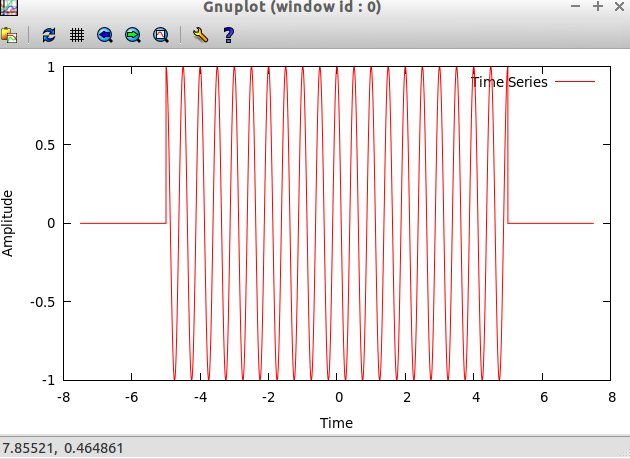
\includegraphics[width=0.75\columnwidth]{T5} % Example image
\end{center}
Cause the following time-series figure too oscillating to show, then we only demonstrate the spectrum.
\begin{center}
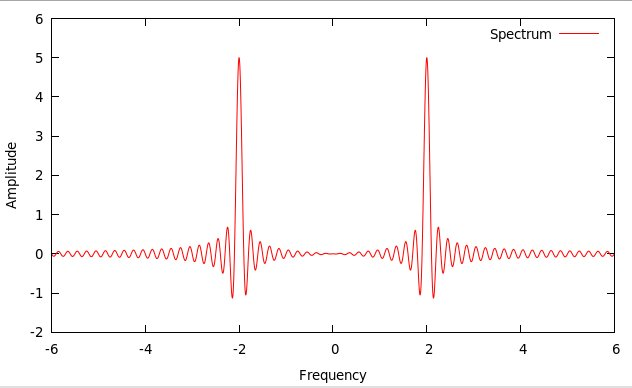
\includegraphics[width=0.75\columnwidth]{F2} % Example image
\end{center}
}
\newpage
\problemAnswer{
\subsection{$T\times f_0 =100, T = 5, f_0 =20 $}
\begin{center}
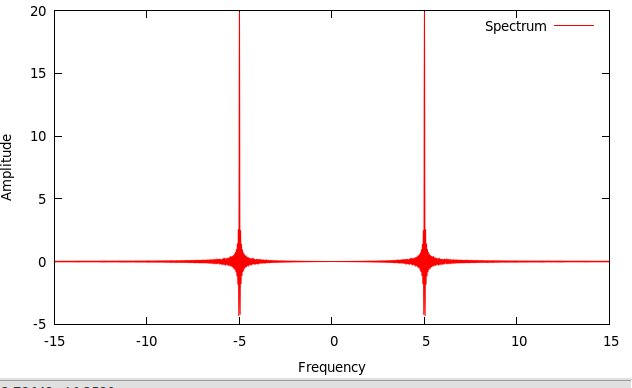
\includegraphics[width=0.75\columnwidth]{T5F20} % Example image
\end{center}
\subsection{$T\times f_0 =1000, T = 20, f_0 =50 $}
\begin{center}
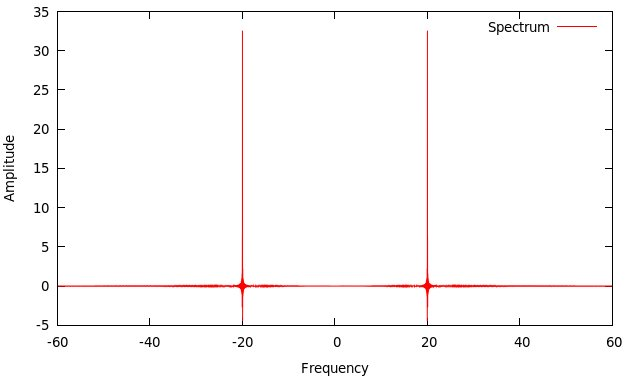
\includegraphics[width=0.75\columnwidth]{T20F50} % Example image
\end{center}
}
\newpage
\problemAnswer{
\section{c.}
As we can find that when $T\times f_0$ get larger, the spectrum gets thinner. The original sinc function gradually become impulse function.
\begin{align*}
\lim_{\tau \rightarrow \infty} \tau sinc(f\tau) = \delta(f)
\end{align*}
\begin{center}
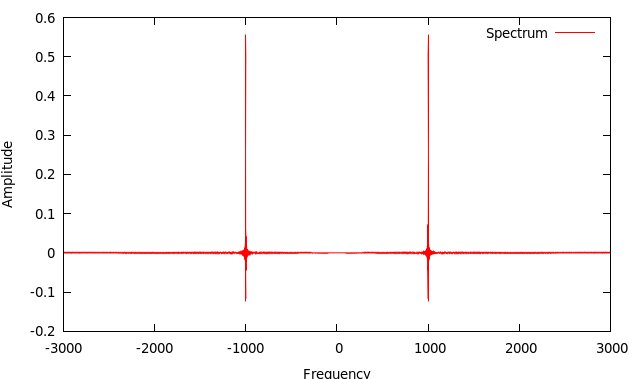
\includegraphics[width=0.75\columnwidth]{T1000F1000} % Example image
\end{center}
}
\end{homeworkProblem}

\begin{homeworkProblem}
Prove the frequency convolution theory\\
\problemAnswer{
\section{a.}
\begin{align*}
\mathcal{F}\{x(t)h(t)\} & = \int_{-\infty}^\infty x(t)h(t)\mathrm{e}^{-j\omega t}\,\mathrm{d}t \\
						& = \int_{-\infty}^\infty [\frac{1}{2\pi}\int_{-\infty}^\infty X(j\omega_1)\mathrm{e}^{j\omega_1 t}\,\mathrm{d}t] h(t)\mathrm{e}^{-j\omega t}\,\mathrm{d}t \\
						& = \frac{1}{2\pi} \int_{-\infty}^\infty X(j\omega_1)[\int_{-\infty}^\infty h(t)\mathrm{e}^{j\omega_1 t}\mathrm{e}^{-j\omega t}\,\mathrm{d}t] \,\mathrm{d}\omega \\
						& = \frac{1}{2\pi} \int_{-\infty}^\infty X(j\omega_1)[\int_{-\infty}^\infty h(t)\mathrm{e}^{-j(\omega-\omega_1)t}\,\mathrm{d}t] \,\mathrm{d}\omega  \\
						& = \frac{1}{2\pi} \int_{-\infty}^\infty X(j\omega_1) H(j(\omega-\omega_1))\,\mathrm{d}\omega \\
						& = X(f) * H(f)
\end{align*}

\section{b.}
Show the Associativity 
\begin{align*}
(f_1*f_2)*f_3 &=  \int_{-\infty}^\infty\int_{-\infty}^\infty f_1(\tau_1)f_2(\tau_2)f_3((t-\tau_1)-\tau_2)d\tau_1d\tau_2 \\
&=\int_{-\infty}^\infty\int_{-\infty}^\infty f_1(\tau_1)f_2((\tau_1+\tau_2)-\tau_1)f_3(t-(\tau_1+\tau_2))d\tau_1d\tau_2 
\end{align*}
That we can find $\tau_3 = \tau_1 + \tau_3$
\begin{align*}
&=\int_{-\infty}^\infty f_1(\tau_1)[\int_{-\infty}^\infty f_2(\tau_2)f_3(t-\tau_2)d\tau_2]d\tau_1 \\
&=f_1*(f_2*f_3)
\end{align*}
}
\end{homeworkProblem}

\section{Appendix Code}
\lstinputlisting[language=c]{spectrum.c}


%x(t) &= \sum_{k=-\infty}^{\infty}c_ke^{k2\pi f_0t} \\
% &= c_0 + \frac{2}{\pi}\sum_{k=1}^{\infty}[\frac{1}{j\pi(2k-1)}e^{j(2k-1)\omega_0 t}+\frac{1}{-j\pi(2k-1)}e^{-j(2k-1)\omega_0 t}] \\
% & = \frac{1}{2} +  \frac{2}{\pi}\sum_{k=1}^{\infty}\frac{sin((2k-1)\omega_0 t)}{2k-1}
%----------------------------------------------------------------------------------------
%	PROBLEM 2
%----------------------------------------------------------------------------------------

%----------------------------------------------------------------------------------------

\end{document}
